\tableofcontents
\section*{Предисловие}
При выполнении данной лабораторной работы было решено использовать 
\href{https://python-control.readthedocs.io/en/0.9.4/}{Python Control Systems Library}.
Данный инструмент является альтернативой Matlab, адаптированной для использования на 
языке Python и предоставляет широкий функционал для анализа и моделирования систем,
а также синтеза регуляторов для управления.

Полный листинг моделирования систем представлен в \href{https://github.com/diuzhevVlad/control-theory-itmo-fall-2023/blob/main/Lab11/Lab11.ipynb}{jupyter notebook} на GitHub.

\pagebreak

\section{Синтез $H_2$-регулятора по состоянию}
Рассмотрим систему:

\begin{equation}
    \begin{cases}
        \dot{x} = Ax + B_1w + B_2u \\
        y = C_1x + D_1w\\
        z = C_2x + D_2u
    \end{cases}
\end{equation}

Можем синтезировать $H_2$-регулятор по состоянию ($u=Kx$) следующим образом:
\begin{equation}
    \begin{cases}
        A^TQ + QA + C_2^TC_2 - QB_2(D_2^TD_2)^{-1}B_2^TQ=0 \\
        K = -(D_2^TD_2)^{-1}B_2^TQ
    \end{cases}
\end{equation}

\begin{equation*}
    A = \begin{bmatrix}
        0 & 1 \\
        0 & 0
    \end{bmatrix},
    B_1 = \begin{bmatrix}
        1 & 0 & 0 \\
        0 & 1 & 0
    \end{bmatrix},
    B_2 = \begin{bmatrix}
        0 \\ 1
    \end{bmatrix},
    C_1 = \begin{bmatrix}
        1 & 0
    \end{bmatrix}
    D_1 = \begin{bmatrix}
        0 & 0 & 1
    \end{bmatrix}
\end{equation*}
Моделирование систем проведем при $w = [sin(t), sin(2t), 1]^T$.
Зададимся двумя вариантами регулируемого выхода $z$:
\subsection{1 вариант}
\begin{equation*}
    C_2 = \begin{bmatrix}
        2 & 0 \\
        0 & 0
    \end{bmatrix}, 
    D_2 = \begin{bmatrix}
        0 \\ 1
    \end{bmatrix},
    K = \begin{bmatrix}
        -2 & -2
    \end{bmatrix}
\end{equation*}
Матрица передаточных функций:
\begin{equation*}
    W = 
    \begin{bmatrix}
        \frac{2s+4}{s^2+2s+2} & \frac{2}{s^2+2s+2} & 0 \\
        \frac{-2s}{s^2+2s+2} & \frac{-2s-2}{s^2+2s+2} & 0
    \end{bmatrix}
\end{equation*}

\begin{equation*}
    ||W(j\omega)||_{H_2} = 2.45, ||W(j\omega)||_{H_\infty} = 2.58
\end{equation*}

Графики анализа данной системы представленны на рисунках \ref{fig:task1_1_1}, \ref{fig:task1_1_2}, \ref{fig:task1_1_3}, \ref{fig:task1_1_4}.


\subsection{2 вариант}
\begin{equation*}
    C_2 = \begin{bmatrix}
        2 & 0 \\
        0 & 1
    \end{bmatrix}, 
    D_2 = \begin{bmatrix}
        2 \\ 0
    \end{bmatrix},
    K = \begin{bmatrix}
        -1 & -1.5
    \end{bmatrix}
\end{equation*}
Матрица передаточных функций:
\begin{equation*}
    W = 
    \begin{bmatrix}
        \frac{3}{s^2+1.5s+1} & \frac{-3s}{s^2+1.5s+1} & 0 \\
        \frac{-1}{s^2+1.5s+1} & \frac{s}{s^2+1.5s+1} & 0
    \end{bmatrix}
\end{equation*}

\begin{equation*}
    ||W(j\omega)||_{H_2} = 2.58, ||W(j\omega)||_{H_\infty} = 3.32
\end{equation*}

Графики анализа данной системы представленны на рисунках \ref{fig:task1_2_1}, \ref{fig:task1_2_2}, \ref{fig:task1_2_3}, \ref{fig:task1_2_4}.


\subsection{Графики}
\begin{figure}[]
    \centering
    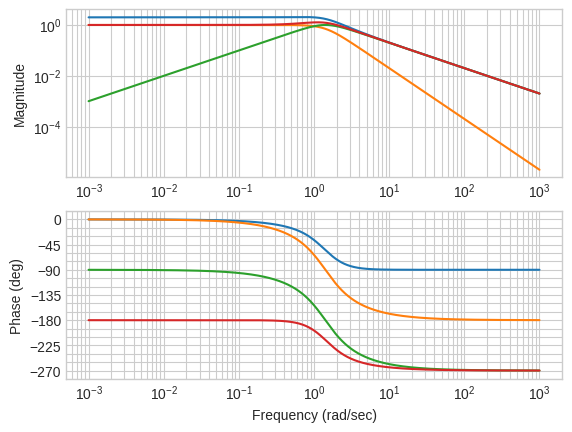
\includegraphics[width=300px]{task_1_mfc_1.png}
    \caption{\label{fig:task1_1_1}Задание 1. Вариант 1. Компоненты матрицы АЧХ и ФЧХ.}
\end{figure}

\begin{figure}[]
    \centering
    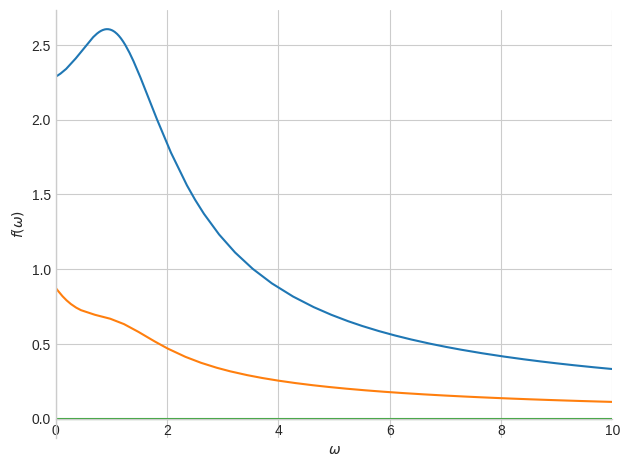
\includegraphics[width=300px]{task_1_svd_1.png}
    \caption{\label{fig:task1_1_2}Задание 1. Вариант 1. Сингулярные числа.}
\end{figure}

\begin{figure}[]
    \centering
    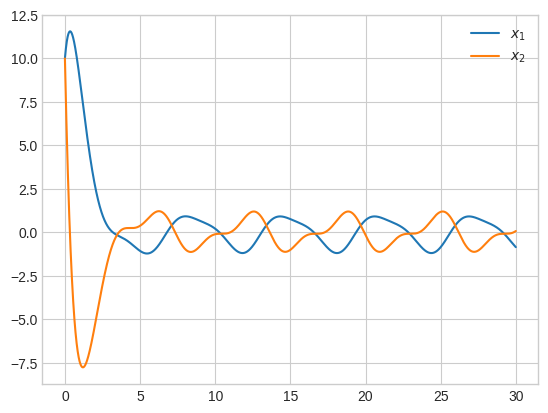
\includegraphics[width=300px]{task_1_x_1.png}
    \caption{\label{fig:task1_1_3}Задание 1. Вариант 1. Вектор состояния системы.}
\end{figure}

\begin{figure}[]
    \centering
    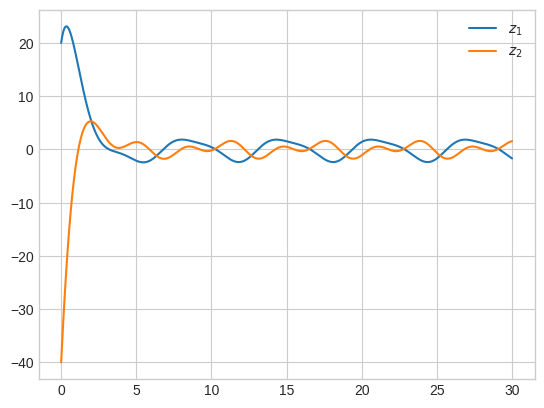
\includegraphics[width=300px]{task_1_z_1.png}
    \caption{\label{fig:task1_1_4}Задание 1. Вариант 1. Регулируемый выход системы.}
\end{figure}

\begin{figure}[]
    \centering
    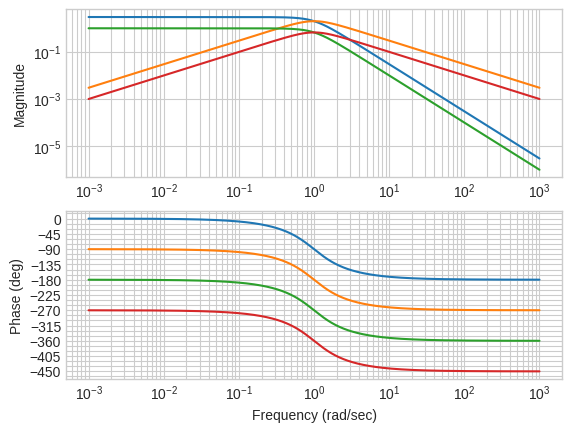
\includegraphics[width=300px]{task_1_mfc_2.png}
    \caption{\label{fig:task1_2_1}Задание 1. Вариант 2. Компоненты матрицы АЧХ и ФЧХ.}
\end{figure}

\begin{figure}[]
    \centering
    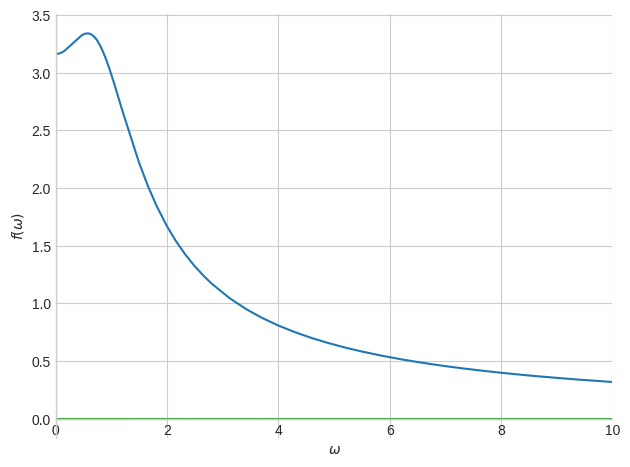
\includegraphics[width=300px]{task_1_svd_2.png}
    \caption{\label{fig:task1_2_2}Задание 1. Вариант 2. Сингулярные числа.}
\end{figure}

\begin{figure}[]
    \centering
    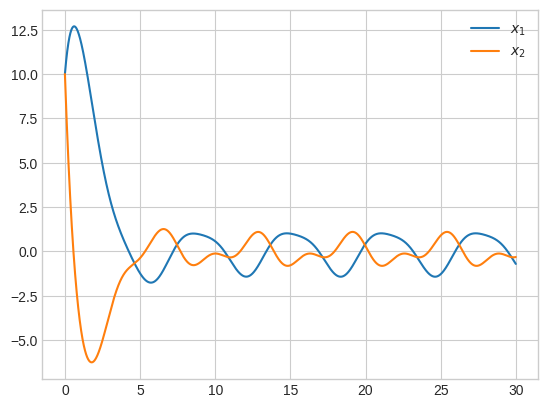
\includegraphics[width=300px]{task_1_x_2.png}
    \caption{\label{fig:task1_2_3}Задание 1. Вариант 2. Вектор состояния системы.}
\end{figure}

\begin{figure}[]
    \centering
    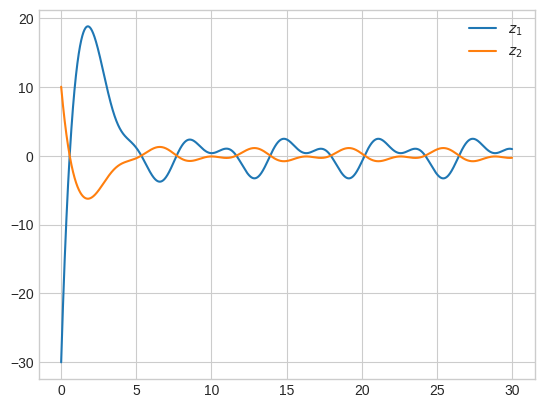
\includegraphics[width=300px]{task_1_z_2.png}
    \caption{\label{fig:task1_2_4}Задание 1. Вариант 2. Регулируемый выход системы.}
\end{figure}

\pagebreak

\section{Синтез $H_2$-регулятора по выходу}

Дополним систему наблюдателем:

\begin{equation}
    \begin{cases}
        \dot{\hat{x}} = A\hat{x} + B_2u + L(\hat{y} - y)\\
        \hat{y} = C_1\hat{x} \\
        \hat{z} = C_2\hat{x}
    \end{cases}
\end{equation}

Можем синтезировать $H_2$-наблюдатель следующим образом:
\begin{equation}
    \begin{cases}
        AP + PA^T + B_1B_1^T - PC_1^T(D_1D_1^T)^{-1}C_1P = 0\\
        L = -PC_1^T(D_1D_1^T)^{-1}
    \end{cases}
\end{equation}

Представим систему в виде:
\begin{equation}
    \begin{cases}
        \begin{bmatrix}
            \dot{x} \\ \dot{e}
        \end{bmatrix} =
        \begin{bmatrix}
            A + B_2K & -B_2K \\
            0 & A + LC_1
        \end{bmatrix} \begin{bmatrix} x \\ e\end{bmatrix} +
        \begin{bmatrix}
            B_1 \\ LD_1 + B_1
        \end{bmatrix}w \\

        z = \begin{bmatrix}
            C_2 + D_2K & -D_2K
        \end{bmatrix} \begin{bmatrix} x \\ e\end{bmatrix}
    \end{cases}
\end{equation}

Моделирование систем проведем при $w = [sin(t), sin(2t), 0.5sin(t)]^T$.
Зададимся двумя вариантами регулируемого выхода $z$:
\subsection{1 вариант}
\begin{equation*}
    C_2 = \begin{bmatrix}
        2 & 0 \\
        0 & 0
    \end{bmatrix}, 
    D_2 = \begin{bmatrix}
        0 \\ 1
    \end{bmatrix},
    K = \begin{bmatrix}
        -2 & -2
    \end{bmatrix},
    L = \begin{bmatrix}
        -1.73 & -1
    \end{bmatrix}^T
\end{equation*}
Матрица передаточных функций:
\begin{equation*}
    W = 
    \begin{bmatrix}
        \frac{2s^3+7.46s^2+12.93s}{s^4 + 3.73s^3 +6.64s^2 + 5.46s + 2} & \frac{2s^2+7.46s+12.93}{s^4 + 3.73s^3 +6.64s^2 + 5.46s + 2} & \frac{-10.93s -4}{s^4 + 3.73s^3 +6.64s^2 + 5.46s + 2} \\
        \frac{-5.46s^2-2s}{s^4 + 3.73s^3 +6.64s^2 + 5.46s + 2} & \frac{-5.46s -2}{s^4 + 3.73s^3 +6.64s^2 + 5.46s + 2} & \frac{-5.46s^3-2s^2}{s^4 + 3.73s^3 +6.64s^2 + 5.46s + 2}
    \end{bmatrix}
\end{equation*}

\begin{equation*}
    ||W(j\omega)||_{H_2} = 5.27, ||W(j\omega)||_{H_\infty} = 7.21
\end{equation*}

Графики анализа данной системы представленны на рисунках \ref{fig:task2_1_1}, \ref{fig:task2_1_2}, \ref{fig:task2_1_3}, \ref{fig:task2_1_4}.

\subsection{2 вариант}
\begin{equation*}
    C_2 = \begin{bmatrix}
        2 & 0 \\
        0 & 2
    \end{bmatrix}, 
    D_2 = \begin{bmatrix}
        1 \\ 1
    \end{bmatrix},
    K = \begin{bmatrix}
        -1.41 & -2.19
    \end{bmatrix},
    L = \begin{bmatrix}
        -1.73 & -1
    \end{bmatrix}^T
\end{equation*}
Матрица передаточных функций:
\begin{equation*}
    W = 
    \begin{bmatrix}
        \frac{2s^3+3.12s^2+11.03s}{s^4 + 3.92s^3 + 6.22s^2 + 4.64s + 1.41} & \frac{2s^2+3.21s+11.03}{s^4 + 3.92s^3 + 6.22s^2 + 4.64s + 1.41} & \frac{-4.64s^3-1.41s^2-9.29s -2.82}{s^4 + 3.92s^3 + 6.22s^2 + 4.64s + 1.41} \\
        \frac{-4.64s^2-10.71s-2.82}{s^4 + 3.92s^3 + 6.22s^2 + 4.64s + 1.41} & \frac{2s^3 + 7.85s^2+7.79s-1.41}{s^4 + 3.92s^3 + 6.22s^2 + 4.64s + 1.41} & \frac{-4.46s^3-10.71s^2-2.82s}{s^4 + 3.92s^3 + 6.22s^2 + 4.64s + 1.41}
    \end{bmatrix}
\end{equation*}

\begin{equation*}
    ||W(j\omega)||_{H_2} = 5.74, ||W(j\omega)||_{H_\infty} = 8.43
\end{equation*}

Графики анализа данной системы представленны на рисунках \ref{fig:task2_2_1}, \ref{fig:task2_2_2}, \ref{fig:task2_2_3}, \ref{fig:task2_2_4}.

\subsection{Графики}
\begin{figure}[]
    \centering
    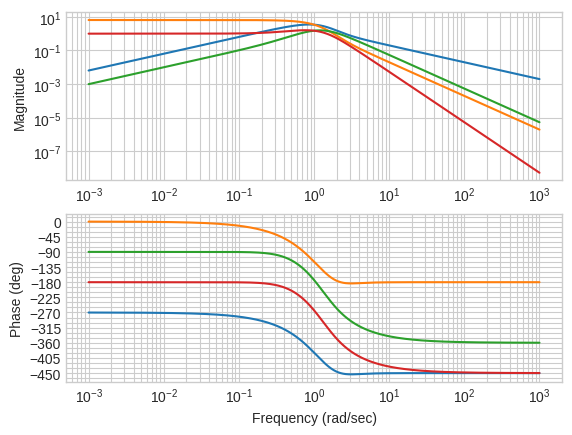
\includegraphics[width=300px]{task_2_mfc_1.png}
    \caption{\label{fig:task2_1_1}Задание 2. Вариант 1. Компоненты матрицы АЧХ и ФЧХ.}
\end{figure}

\begin{figure}[]
    \centering
    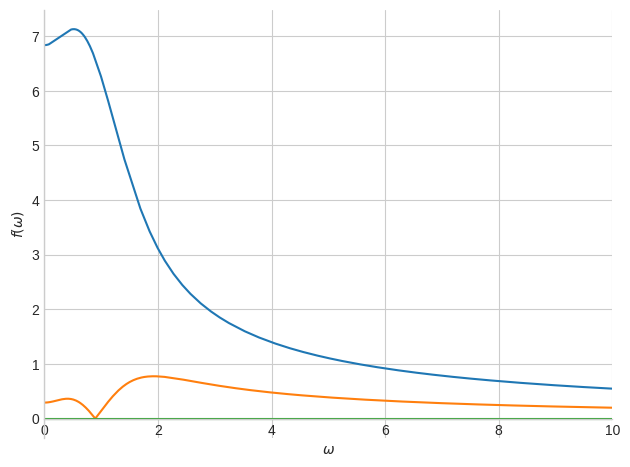
\includegraphics[width=300px]{task_2_svd_1.png}
    \caption{\label{fig:task2_1_2}Задание 2. Вариант 1. Сингулярные числа.}
\end{figure}

\begin{figure}[]
    \centering
    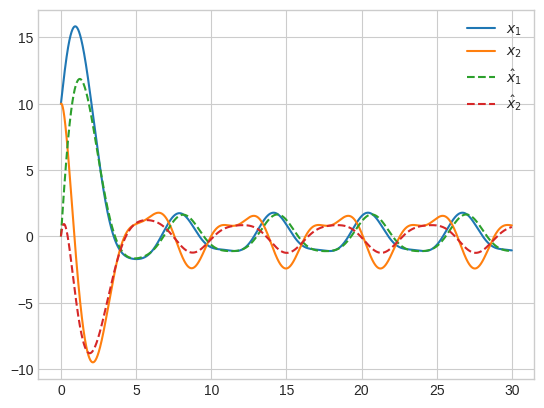
\includegraphics[width=300px]{task_2_x_1.png}
    \caption{\label{fig:task2_1_3}Задание 2. Вариант 1. Вектор состояния системы.}
\end{figure}

\begin{figure}[]
    \centering
    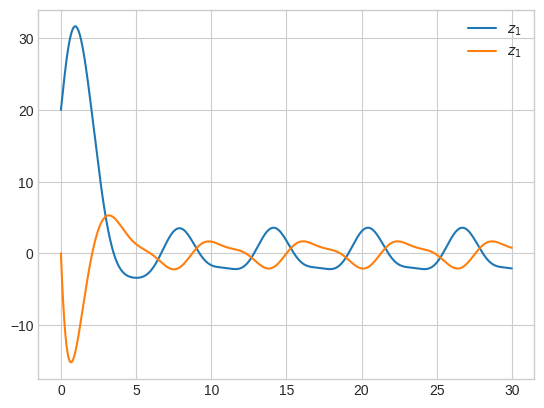
\includegraphics[width=300px]{task_2_z_1.png}
    \caption{\label{fig:task2_1_4}Задание 2. Вариант 1. Регулируемый выход системы.}
\end{figure}

\begin{figure}[]
    \centering
    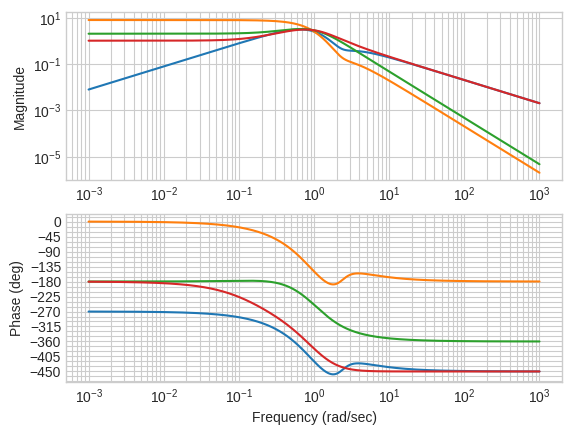
\includegraphics[width=300px]{task_2_mfc_2.png}
    \caption{\label{fig:task2_2_1}Задание 2. Вариант 2. Компоненты матрицы АЧХ и ФЧХ.}
\end{figure}

\begin{figure}[]
    \centering
    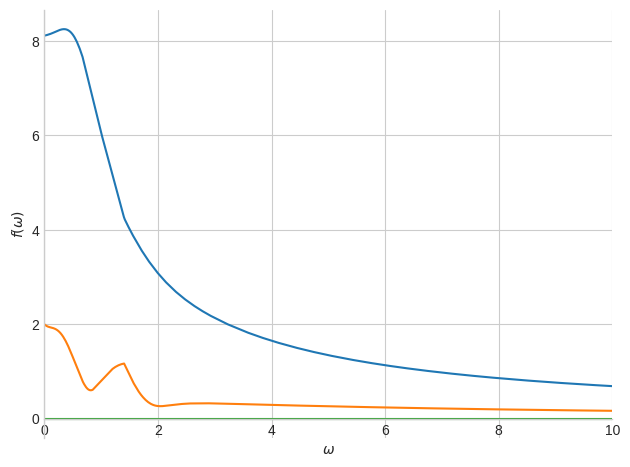
\includegraphics[width=300px]{task_2_svd_2.png}
    \caption{\label{fig:task2_2_2}Задание 2. Вариант 2. Сингулярные числа.}
\end{figure}

\begin{figure}[]
    \centering
    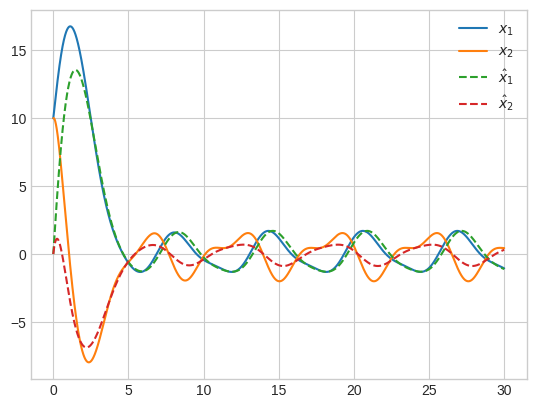
\includegraphics[width=300px]{task_2_x_2.png}
    \caption{\label{fig:task2_2_3}Задание 2. Вариант 2. Вектор состояния системы.}
\end{figure}

\begin{figure}[]
    \centering
    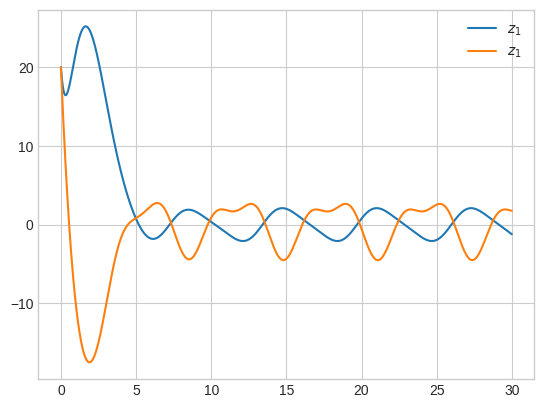
\includegraphics[width=300px]{task_2_z_2.png}
    \caption{\label{fig:task2_2_4}Задание 2. Вариант 2. Регулируемый выход системы.}
\end{figure}

\pagebreak

\section{Синтез $H_\infty$-регулятора по состоянию}

Рассмотрев систему (1) можем синтезировать $H_\infty$-регулятор по состоянию:

\begin{equation}
    \begin{cases}
        A^TQ + QA +C_2^TC_2 - QB_2(D_2^TD_2)^{-1}B_2^TQ + \gamma^{-2}QB_1B_1^TQ=0 \\
        K = -(D_2^TD_2)^{-1}B_2^TQ
    \end{cases}
\end{equation}

Изменим матрицы системы следующим образом:
\begin{equation*}
    C_1 = \begin{bmatrix}
        1 & 0
    \end{bmatrix},
    C_2 = \begin{bmatrix}
        2 & 0 \\ 0 & 0
    \end{bmatrix},
    D_2 = \begin{bmatrix}
        0 \\ 1
    \end{bmatrix}
\end{equation*}

\begin{table}[h!]
    \centering
    \begin{tabular}{| l | l | l | l |} 
        \hline
        $\gamma$ & $K$ & $||W(j\omega)||_{H_2}$ & $||W(j\omega)||_{H_\infty}$ \\  
        \hline\hline
        $1.65$ & $\begin{bmatrix} -32.89 & -27.05 \end{bmatrix}$ & $5.98$ & $1.61$ \\ 
        \hline
        $3$ & $\begin{bmatrix} -2.77 & -2.68 \end{bmatrix}$ & $2.49$ & $2.34$ \\
        \hline
        $10$ & $\begin{bmatrix} -2.05 & -2.04 \end{bmatrix}$ & $2.44$ & $2.64$ \\
        \hline
       \end{tabular}
    \caption{Результаты синтеза регулятора с заданными $\gamma$.}
    \label{table:1}
\end{table}

Графики анализа системы, замкнутой регулятором при различных $\gamma$ приведены ниже (рис. 17-24):

\begin{figure}[]
    \centering
    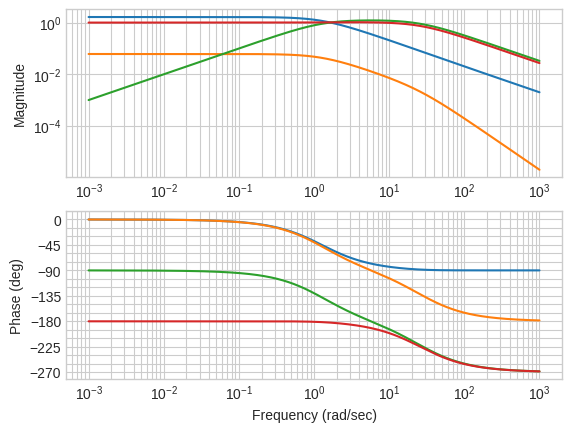
\includegraphics[width=300px]{task_3_mfc_1.png}
    \caption{\label{fig:task3_1_1}Задание 3. $\gamma = 1.65$. Компоненты матрицы АЧХ и ФЧХ.}
\end{figure}

\begin{figure}[]
    \centering
    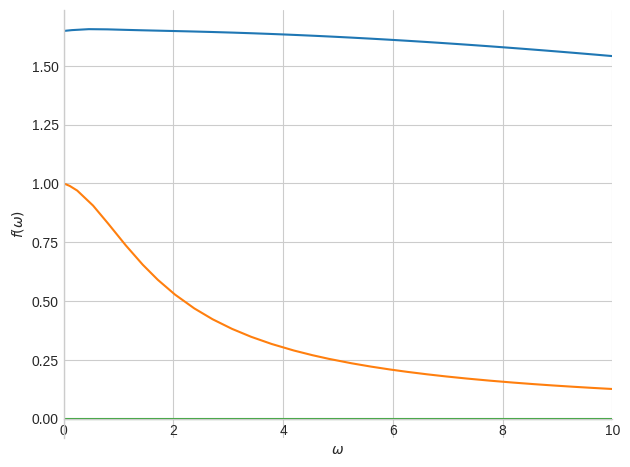
\includegraphics[width=300px]{task_3_svd_1.png}
    \caption{\label{fig:task3_1_2}Задание 3. $\gamma = 1.65$. Сингулярные числа.}
\end{figure}

\begin{figure}[]
    \centering
    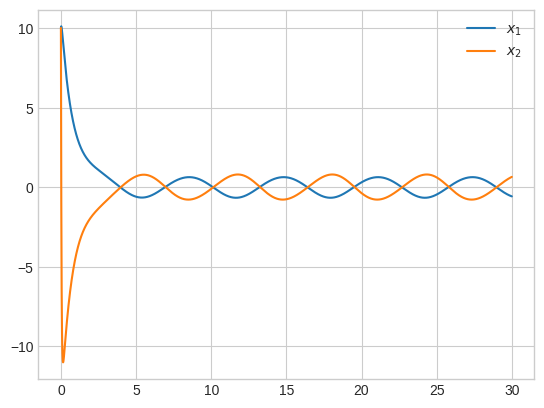
\includegraphics[width=300px]{task_3_x_1.png}
    \caption{\label{fig:task3_1_3}Задание 3. $\gamma = 1.65$. Вектор состояния системы.}
\end{figure}

\begin{figure}[]
    \centering
    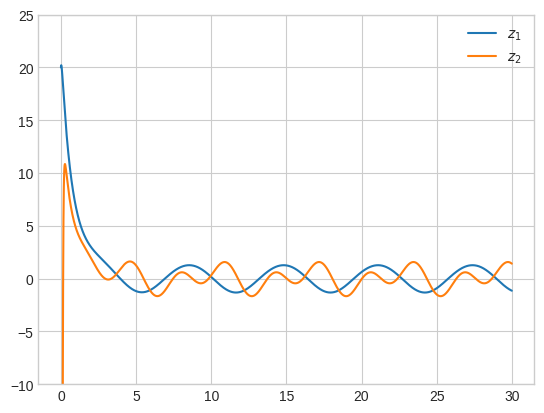
\includegraphics[width=300px]{task_3_z_1.png}
    \caption{\label{fig:task3_1_4}Задание 3. $\gamma = 1.65$. Регулируемый выход системы.}
\end{figure}

\begin{figure}[]
    \centering
    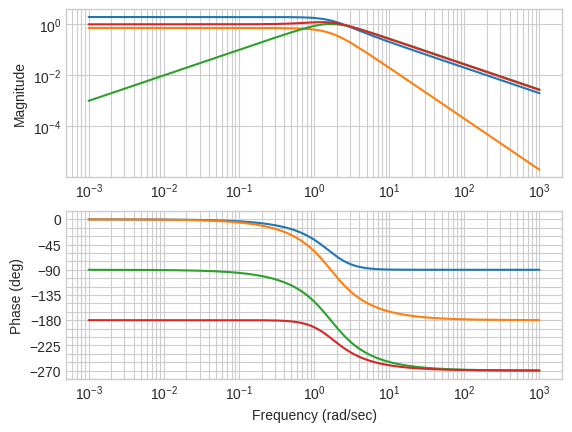
\includegraphics[width=300px]{task_3_mfc_2.png}
    \caption{\label{fig:task3_2_1}Задание 3. $\gamma = 3$. Компоненты матрицы АЧХ и ФЧХ.}
\end{figure}

\begin{figure}[]
    \centering
    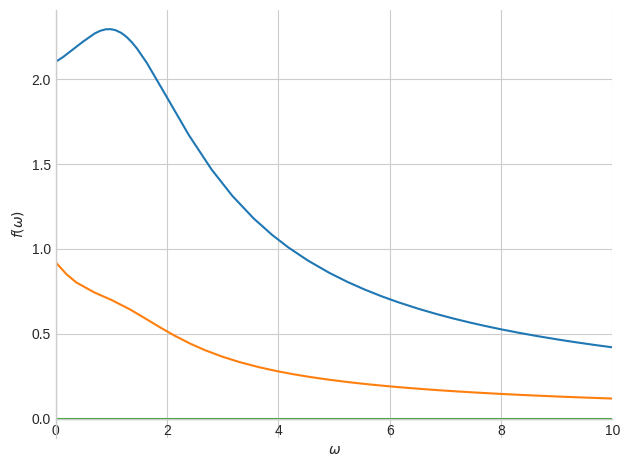
\includegraphics[width=300px]{task_3_svd_2.png}
    \caption{\label{fig:task3_2_2}Задание 3. $\gamma = 3$. Сингулярные числа.}
\end{figure}

\begin{figure}[]
    \centering
    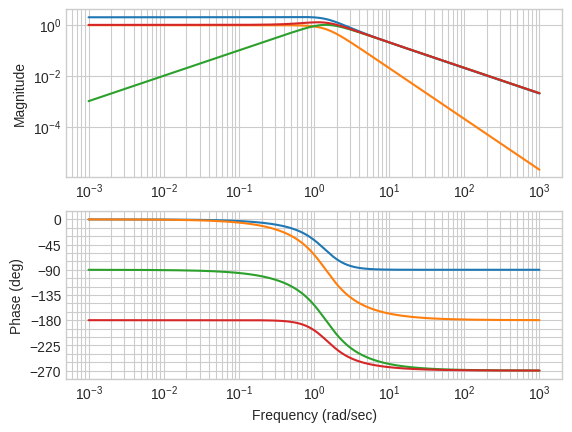
\includegraphics[width=300px]{task_3_mfc_3.png}
    \caption{\label{fig:task3_1_1}Задание 3. $\gamma = 10$. Компоненты матрицы АЧХ и ФЧХ.}
\end{figure}

\begin{figure}[]
    \centering
    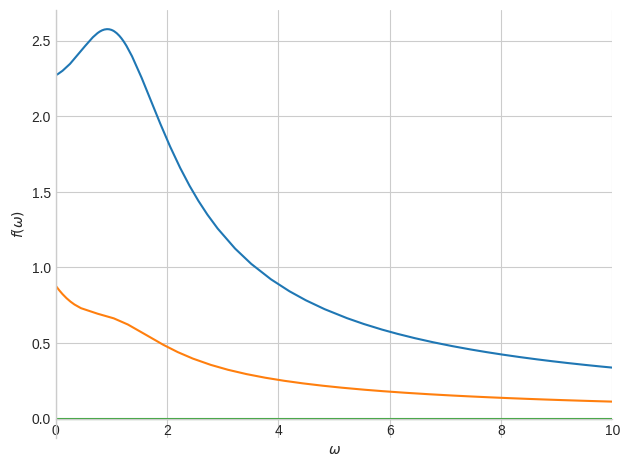
\includegraphics[width=300px]{task_3_svd_3.png}
    \caption{\label{fig:task3_1_2}Задание 3. $\gamma = 10$. Сингулярные числа.}
\end{figure}

\pagebreak

\section{Синтез $H_\infty$-регулятора по выходу}

Рассмотрев системы (1) и (3) можем синтезировать $H_\infty$-регулятор по выходу (совместно с наблюдателем) следующим образом:
\begin{equation}
    \begin{cases}
        AP + PA^T + B_1B_1^T - PC_1^T(D_1D_1^T)^{-1}C_1P = 0 \\
        L = - PC_1^T(D_1^TD_1)^{-1} \\
        A^TQ + QA + C_2^TC_2 - QB_2(D_2^TD_2)^{-1}B_2^TQ = 0 \\
        K = -(D_2^TD_2)^{-1}B_2^TQ
    \end{cases}
\end{equation}

Представим систему в виде:
\begin{equation}
    \begin{cases}
        \begin{bmatrix}
            \dot{x} \\ \dot{e}
        \end{bmatrix} =
        \begin{bmatrix}
            A + B_2K & -B_2K \\
            -(LD_1B_1)\gamma^{-2}B_1^TQ & A + LC_1 + (LD_1B_1)\gamma^{-2}B_1^TQ
        \end{bmatrix} \begin{bmatrix}
            x \\ e
        \end{bmatrix} +
        \begin{bmatrix}
            B_1 \\
            LD_1 + B_1
        \end{bmatrix}w \\
        z = \begin{bmatrix}
            C_2 +D_2K & -D_2K
        \end{bmatrix}\begin{bmatrix}
            x \\ e
        \end{bmatrix}
    \end{cases}
\end{equation}

\begin{table}[h!]
    \centering
    \begin{tabular}{| l | l | l | l | l |} 
        \hline
        $\gamma$ & $K$ & $L$ & $||W(j\omega)||_{H_2}$ & $||W(j\omega)||_{H_\infty}$ \\  
        \hline\hline
        $5.2$ & $\begin{bmatrix} -2.41 & -3.06 \end{bmatrix}$ & $\begin{bmatrix} -83.74 & -74.41 \end{bmatrix}^T$ & $33.37$ & $5.19$ \\ 
        \hline
        $7$ & $\begin{bmatrix} -2.21 & -2.94 \end{bmatrix}$ & $\begin{bmatrix} -3.32 & -2.38 \end{bmatrix}^T$ & $7.12$ & $6.48$ \\
        \hline
        $10$ & $\begin{bmatrix} -2.09 & -2.88 \end{bmatrix}$ & $\begin{bmatrix} -2.21 & -1.42 \end{bmatrix}^T$ & $6.37$ & $7.41$ \\
        \hline
       \end{tabular}
    \caption{Результаты синтеза полного регулятора с заданными $\gamma$.}
    \label{table:2}
\end{table}

Графики анализа системы, замкнутой регулятором при различных $\gamma$ приведены на рисунках 25-30:

\begin{figure}[]
    \centering
    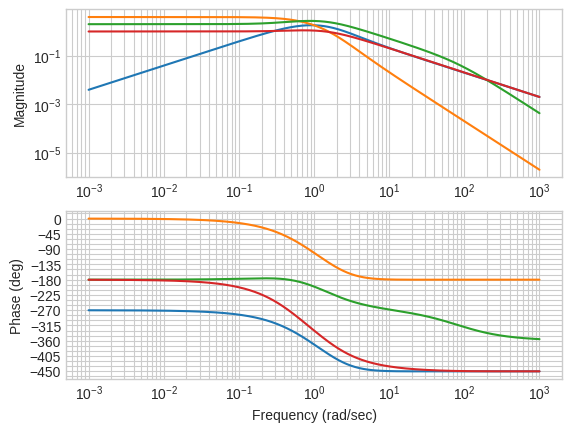
\includegraphics[width=300px]{task_4_mfc_1.png}
    \caption{\label{fig:task4_1_1}Задание 4. $\gamma = 5.2$. Компоненты матрицы АЧХ и ФЧХ.}
\end{figure}

\begin{figure}[]
    \centering
    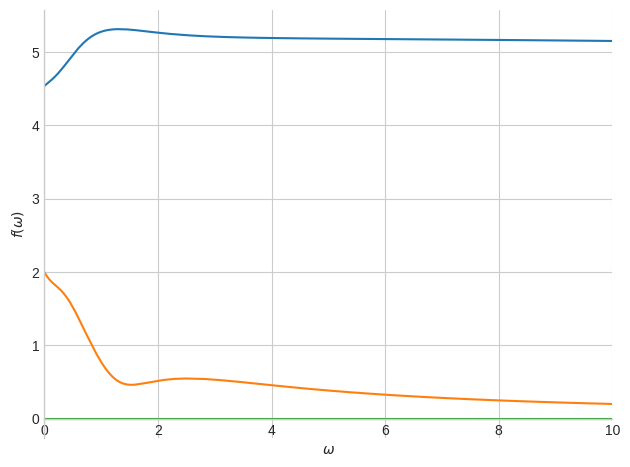
\includegraphics[width=300px]{task_4_svd_1.png}
    \caption{\label{fig:task4_1_2}Задание 4. $\gamma = 5.2$. Сингулярные числа.}
\end{figure}

\begin{figure}[]
    \centering
    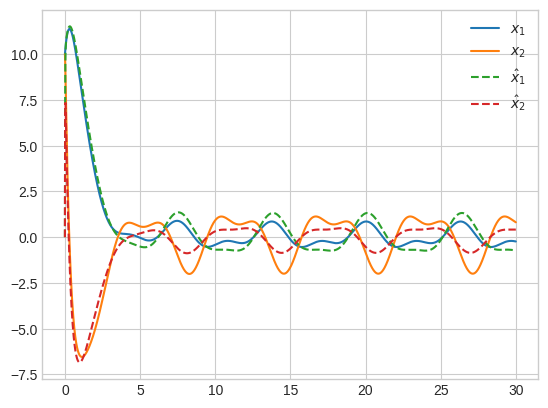
\includegraphics[width=300px]{task_4_x_1.png}
    \caption{\label{fig:task4_1_3}Задание 4. $\gamma = 5.2$. Вектор состояния системы.}
\end{figure}

\begin{figure}[]
    \centering
    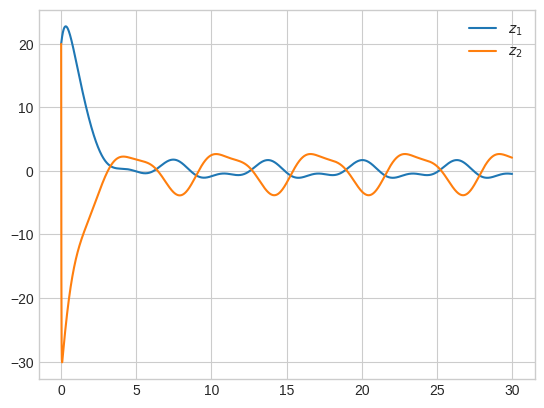
\includegraphics[width=300px]{task_4_z_1.png}
    \caption{\label{fig:task4_1_4}Задание 4. $\gamma = 5.2$. Регулируемый выход системы.}
\end{figure}

\begin{figure}[]
    \centering
    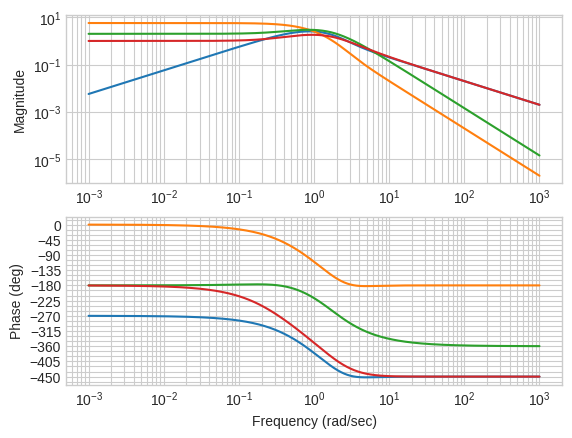
\includegraphics[width=300px]{task_4_mfc_2.png}
    \caption{\label{fig:task4_2_1}Задание 4. $\gamma = 7$. Компоненты матрицы АЧХ и ФЧХ.}
\end{figure}

\begin{figure}[]
    \centering
    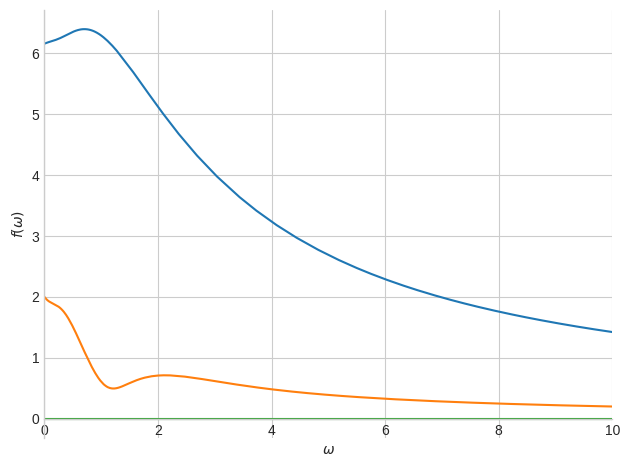
\includegraphics[width=300px]{task_4_svd_2.png}
    \caption{\label{fig:task4_2_2}Задание 4. $\gamma = 7$. Сингулярные числа.}
\end{figure}

\begin{figure}[]
    \centering
    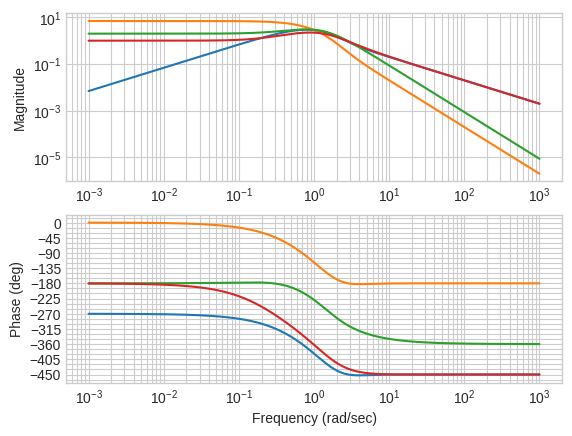
\includegraphics[width=300px]{task_4_mfc_3.png}
    \caption{\label{fig:task4_3_1}Задание 4. $\gamma = 10$. Компоненты матрицы АЧХ и ФЧХ.}
\end{figure}

\begin{figure}[]
    \centering
    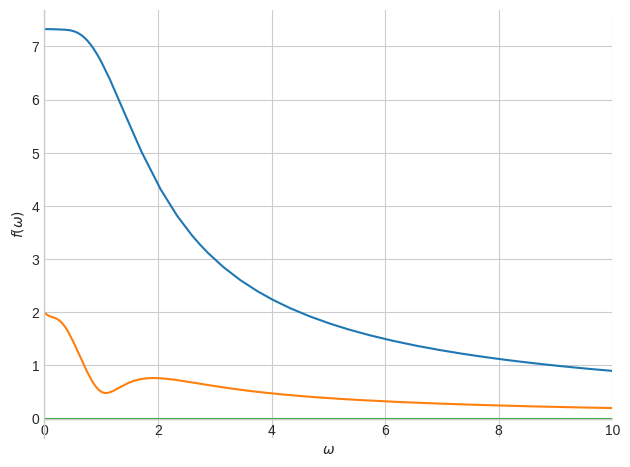
\includegraphics[width=300px]{task_4_svd_3.png}
    \caption{\label{fig:task4_3_2}Задание 4. $\gamma = 10$. Сингулярные числа.}
\end{figure}

\pagebreak

\section{Выводы}
В ходе выполнения данной работы были получены навыки синтеза и исследования методов оптимального управления ($H_2$, $H_\infty$ регуляторов и наблюдателей).
\begin{enumerate}
    \item Наблюдается тенденция взаимоисключающей оптимизации $H_2$ и $H_\infty$ нормы системы.
    \item $H_2$-регуляторы ведут себя в целом жесче (коэффициенты регулирования больше), в то время как для наблюдателей замечена обратная тенденция.
    \item При моделировании систем с внешними воздействиями удавалось добиться установившихся колебаний ошибки в определенной области.
\end{enumerate}
\pagebreak